\chapter{Przegląd algorytmów z literatury}

\section{Wstępne przetwarzanie obrazu}
Pierwszym etapem detekcji pasów ruchu drogowego jest konwersja obrazu kolorowego w~formacie RGB (ang. \textit{Red, Green, Blue} -- czerwony, zielony, niebieski) na~obraz binarny.
Proces ten ma na celu aby wstępnie otrzymać cechy określające dany obraz oraz ułatwić dalsze jego przetwarzanie. W~celu ułatwienia konwersji z kolorowego na binarny, możemy przekonwertować wstępnie obraz do formatu w~skali szarości. 

Każdy piksel w~formacie RGB składa się z trzech kanałów, każdy przyjmuje wartości z~przedziału od~0 do 255, gdzie 0 oznacza brak nasycenia danego koloru, a 255 maksymalne nasycenie.
W skali szarości na jeden piksel przypada tylko jeden kanał przyjmujący wartości od 0 do 255.
Dla obrazu binarnego na jeden piksel również przypada tylko jeden kanał, ale może przyjmować wartości 0 lub 1, gdzie 0~to~brak nasycenia kolorów, a 1 to pełne nasycenie kolorów.
Obraz w skali szarości z obrazu w~formacie RGB można otrzymać, np. wyznaczając średnią wartość trzech kanałów dla każdego z pikseli \cite{4}, lub poprzez wykorzystanie składowej L z formatu HSL (ang. \textit{Hue, Saturation, Lightness} -- odcień, saturacja, jasność) \cite{reichenbach_comparison}.


Jednym z metod konwersji obrazu ze skali szarości do binarnego, który zaproponowano w~pracy \cite{4}, jest zwiększenie kontrastu dzięki wykorzystaniu rozciągania histogramu. Następnie korzystając z filtru Sobel'a uwydatnia się krawędzie obiektów, które ma na celu ułatwienie późniejszej detekcji linii pasa ruchu drogowego. Kolejno wykorzystuje się progowanie polegające na przypisywaniu wartości 0 lub 1 do piksela w zależności od tego czy jego wartość jest mniejsza od wartości progu, czy nie. Operator Sobel'a jest zasadniczo operatorem różniczkowania dyskretnego, zwraca pochodne pierunkowe obrazu w ośmiu kierunkach co 45 stopni \cite{3}, \cite{sobel}.


Innym podejściem \cite{reichenbach_comparison} jest wykorzystanie algorytmu Canny Edge Detector w miejscu filtra Sobel'a. Canny Edge łączy w sobie filtr sobela i zdefiniowaną histerezę \cite{cany}. Jeśli wartość gradientu $G$ \eqref{eq:1} piksela jest powyżej ustalonego progu górnego, zaliczany jest do zbioru krawędzi. Gdy jest poniżej ustalonego progu dolnego piksel jest odrzucany. Gdy znajduje się pomiędzy oboma wspomnianymi progami, piksel zostanie zaliczony do zbioru krawędzi jeśli sąsiaduje z pikselem zaklasyfikowanym jako krawędź.

\begin{equation}
G_{x} = \begin{bmatrix} -1 & 0 & +1 \\ -2 & 0 & +2 \\ -1 & 0 & +1 \end{bmatrix}, G_{y} = \begin{bmatrix} -1 & -2 & -1 \\ 0 & 0 & 0 \\ +1 & +2 & +1 \end{bmatrix},
G = \sqrt{ G_{x}^{2} + G_{y}^{2} } \label{eq:1}
\end{equation}

Próg binaryzacji można również dobrać samodzielnie, np. przyjmując, że jego wartość jest równa połowie wartości maksymalnej jaką może mieć piksel \cite{1}. Innym podejściem, zaprezentowanym w~artykule \cite{2}, jest wykorzystanie funkcji entropii lub histogramu.
Histogram obrazu jest sposobem reprezentacji rozkładu wartości piksleli, z~których składa się obraz. 
Może przyjmować formę interpolowanego wykresu, gdzie pozioma oś układu współrzędnych odpowiada za wartość piksela. 
A pionowa oś reprezentuje liczebność punktów o~wartości równej wartości argumentu znajdującego się na~poziomej osi \cite{histogram}.
Na rysunku \ref{fig:entr_hist} przedstawiono zestawienie wykresu danego histogramu oraz wykresu funkcji entropii. 
Funkcje te mają charakterystyczną cechę wspólną. 
Argument dla drugiej największej wartości funkcji entropii jest równy argumentowi dla jakiego histogram przyjmuje wartość maksymalną. Próg binaryzujący znajduje się pomiędzy dwoma największymi wierzchołkami funkcji entropii.

\begin{figure}[h]
	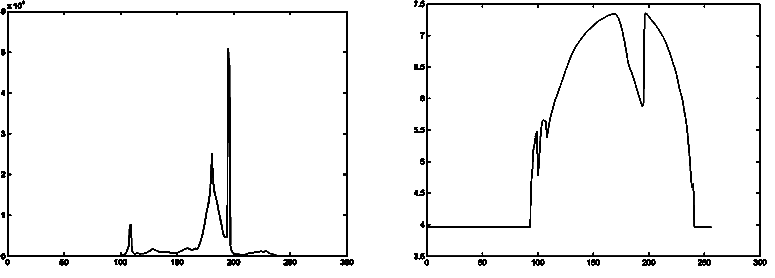
\includegraphics[scale=0.8]{Entropia.png}
	\caption{Porównanie histogramu i funkcji entropii. Źródło: \cite{2}}
	\label{fig:entr_hist}
\end{figure}

\section{Wyznaczanie obszaru zainteresowania}
Pomimo występowania różnorodnych pasów ruchu w rzeczywistości, część ich cech charakterystycznych pozostaje bez zmian.
W wyniku zjawiska perspektywy, czym obiekt jest dalej od kamery tym staje się mniejszy, linie drogowe bliżej kamery, w dolnej części obrazka, są grubsze od tych znajdujących się dalej, w wyższej części obrazu.
To samo dotyczy całego pasa ruchu. W~dolnym obszarze obrazu występuje większy stosunek obiektu pierwszoplanowego, którym jest pas ruchu w~stosunku do~tła, reprezentowanego przez pobocze i obszar poza drogą.
Dodatkowo linie znajdujące się bliżej kamery wakazują na obrazie mniejszą tendencję do nagłej zmiany swojego położenia.
Natomiast nawet lekkie zakręty powodują nagłe przesunięcia się obiektów w~górnej części obrazu.
Podane zależności są charakterystyczne dla obrazów przedstawiających fragment ulicy wzdłuż której porusza się samochód.
Przyczyniło się to powstanie różnych konceptów wyznaczania ROI (ang. \textit{Region Of Interest} -- obszar zainteresowania).
W~pracach \cite{2} i~\cite{4} wykorzystano określenie statycznego obszaru zainteresowania.
ROI jest w kształcie trapezu zwężającego się w kierunku górnej części obrazu \cite{4}.

Wyznaczanie obszaru zainteresowania na obrazie może odbywać w sposób statyczny albo dynamiczny. 
Wyznaczanie statyczne polega na predefiniowanych ograniczeniach, na podstawie których otrzymywany jest obraz przetworzony. 
Dynamiczne odnosi się do sytuacji, w~której wyznaczony obszar zainteresowania zależny jest od danych wejściowych. 
W artykule \cite{vanishing_point} przedstawiono podejście polegające na wyznaczaniu obszaru zainteresowania na podstawie określonego punktu na horyzoncie.
Jest to punkt przecięcia się dwóch prostych, powstałych w skutek przedłużenia linii określających krawędzie drogi. 
Celem wyznaczenia ROI jest pozbycie się jak największej części obrazu, na której nie znajduje się pas ruchu.
Ma to na celu zmniejszenie wpływu tła na działanie algorytmów do detekcji linii.

\section{Wyznaczanie linii drogowych}
W tym etapie skupimy się na detekcji pasów ruchu poprzez wyznaczenie linii na~podstawie obrazu binarnego. 
W~artykule \cite{reichenbach_comparison} wykorzystano w tym celu transformatę Hough'a. 
Jest to metoda wykrywania prostych w~widzeniu komputerowym \cite{hough}.

Prostą znajdującą się na obrazie o współrzędnych kartezjańskich ${x,y}$ można zapisać jako punkt w układzie o współrzędnych $\theta$, $\rho$ \ref{fig:rotheta} (przestrzeń Hough'a) spełniający zależność \eqref{eq:2}, gdzie $\theta$ - kąt nachylenia, $\rho$ - odległość od początku układu współrzędnych.

\begin{equation}
\,x\cos(\theta )+\,y\sin(\theta )=\rho \label{eq:2}
\end{equation}


W celu wyznaczenia pełnego obrazu w przestrzeni Hough'a należy przeiterować po całym przetwarzanym obrazie i dla każdego piksela o wartości 1 (białego) zaznaczyć w układzie $\theta$, $\rho$ wszystkie punkty odpowiadające prostym we współrzędnych ${x,y}$ jakie mogą przechodzić przez ten piksel.

\begin{figure}
	\centering
	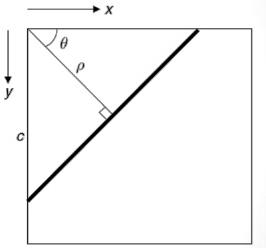
\includegraphics[scale=0.8]{hough_rotheta.png}
	\caption{Graficzne przedstawienie zależności współrzędnych ${x,y}$ i $\theta$, $\rho$. Źródło: \cite{hough_rotheta}}
	\label{fig:rotheta}
\end{figure}

Zakres grubości pasów znajdujących się przykładowo na autostradzie jest ściśle określony przepisami ruchu drogowego. 
Ta zależność została wykorzystana w pracy \cite{4}, gdzie użyto filtru wykrywającego linie ruchu drogowego. Działa on na zasadzie sprawdzania odległości w~poziomie pomiędzy dwoma białymi pikselami. Jeśli mieści się on w ustalonej normie oznacza to, że punkty leżą na linii.
Zakres dobierany jest w~zależności od badanej części obrazu, z zachowaniem właściwości perspektywy \ref{fig:lmps_sobe}. 



\begin{figure}
	\centering
	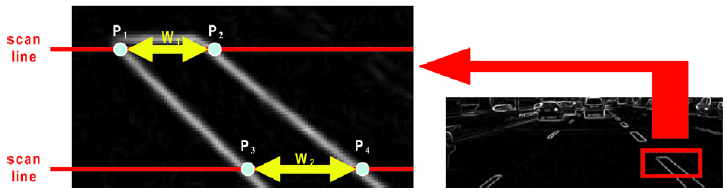
\includegraphics[scale=0.6]{lmps_sobe.png}
	\caption{Zdjęcie przedstawiająca sprawdzanie odległości w poziomie pomiędzy dwoma białymi pikselami. Źródło: \cite{4}}
	\label{fig:lmps_sobe}
\end{figure}

\section{Fuzja obrazu oraz~danych z~mapy}

Postrzeganie otoczenia jest jednym z~głównych wyzwań dla systemów w~pojazdach autonomicznych. 

Przednia kamera w~pojeździe dostarcza informacji o~kluczowych elementach drogi takich jak oznaczenia pasa ruchu i~jego granice. 
Poprawna detekcja przestrzeni, po której auto może się poruszać jest poważnym wyzwaniem ze względu na występowanie wielu pasów ruchu, przecinania się linii.

W artykule \cite{hdmap} podjęto się przeprowadzenia fuzji detekcji pasa ruchu drogowego oraz informacji z~HD (ang. \textit{High Definition} -- wysoka rozdzielczość) mapy. 
Informacja o obecnym położeniu auta zapewniła możliwość wyekstrahowania z~mapy danych o~kształcie drogi na jakiej się znajdował.

Zaproponowane podejście ma znaczącą przewagę nad korzystaniem z~samej kamery, ponieważ jest w~stanie rekompensować skutki takich błędów jak: 
\begin{enumerate}
	\item zmienne warunki oświetlenia, obraz może zawierać nieregularne cienie lub przebłyski,
	\item brak widoczności linii drogowych, naruszona tekstura krawędzi,
	\item nieregularna kolorystycznie nawierzchnia drogowa lub  obiekty ją przysłaniające,
	\item kamera może nie uchwycić całego obszaru, który powinien zostać wykryty, ze względu na krzywiznę drogi.
\end{enumerate}
W~sytuacji, gdy z~obrazu nie da się uzyskać wystarczających informacji przykładowo o~nagłym zakręcie na drodze, dane z~mapy mogą okazać się nieocenione.
